Il grafico della energia di legame media per nucleone commentato nel
precedente paragrafo contiene un certo numero di importanti indicazioni
sulle proprietà della forza nucleare che sono alla base di un primo
modello del nucleo - suggerito da Bohr nel 1935 - fondato essenzialmente
sul \textbf{raggio finito} della interazione nucleare.
Similmente alle
forze intramolecolari a corto raggio nei liquidi, tale fatto determina
una certa analogia tra il comportamento dei nucleoni nel nucleo e le
diverse porzioni di un fluido meccanico incomprimibile, ragione che
giustifica il nome spesso usato di \textbf{modello a goccia}.
Il
suddetto modello ha base \textbf{fenomenologica}; la sola ipotesi
dell'andamento a corto raggio della forza non è sufficiente a
giustificare l'andamento reale

Come accennato, l'energia di legame tende ad assumere rapidamente il
valore medio di circa \(8MeV\) per nucleone (saturazione) il che indica
una energia di legame del nucleo proporzionale al numero di nucleoni \[
	\frac{B}{A} \simeq 8 MeV \qquad B \simeq 8 MeV \times A
\] Ora, se la forza nucleare si comportasse come una forza a lungo
raggio (come le forze gravitazionali o elettromagnetiche) ogni nucleone
interagirebbe con tutti i rimanenti altri per cui dovremmo attenderci
una energia di legame del nucleo tendenzialmente proporzionale al numero
di coppie di nucleoni e dunque quadratica in A \[
	B \propto \frac{A(A-1)}{2} \propto A^{2} \qquad
\] Poiché i dati sulla energia di legame escludono questo tipo di
comportamento, dobbiamo concludere che ogni nucleone del nucleo
interagisce solo con un numero di fisso di nucleoni vicini per cui
concludiamo che l'interazione forte ha un raggio d'azione finito
dell'ordine di grandezza delle dimensioni del nucleone stesso.

Tale conclusione è in perfetto accordo con i dati sulla sezione d'urto
di neutroni su nuclei analizzati in precedenza che indicavano un volume
nucleare proporzionale al numero di nucleoni, ovvero una densità
volumetrica di nucleoni uniforme sul volume nucleare, fatto spiegabile
solo postulando la esistenza di una forza d'interazione tra nucleoni a
corto raggio.

Il primo tentativo di superare questo limite consiste nell'introdurre un
termine \[
	B = a_{v} A
\] dove la costante \(a_{v}\) viene detta \textbf{termine di volume}.Con
un andamento \(B / A\) , però, si finisce per ottenere una sovrastima
del volume.
\begin{marginfigure}
	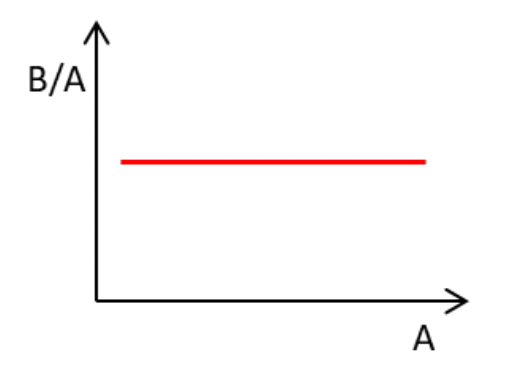
\includegraphics{figs/goccia1}
	%    \caption{This is a margin figure.}
	\label{fig:goccia1}
\end{marginfigure}
La deviazione più rilevante si manifesta per valori piccoli di A dove
l'energia media di legame è molto inferiore a quanto previsto dalla
formula.
Si può allora osservare che, assumendo la forza nucleare a
corto raggio, si deve tenere conto che un nucleone prossimo alla
superficie del nucleo interagirà con un numero di nucleoni inferiore a
quello con cui interagirebbe qualora si trovasse all'interno del nucleo
stesso.
Ciò comporta che i nucleoni superficiali contribuiranno in
misura minore alla energia di legame nucleare di quelli interni al
volume.
Assumendo il nucleo di \textbf{forma sferica}, il numero di
nucleoni prossimi alla superficie sarà proporzionale a \(R^{2}\).
Dalla
trattazione precedente sappiamo che(omettendo il termine di ``skin
nucleare''\,``) \begin{gather*}
	R_{\text{nuc}} = r_{0}A^{1/3}\\
	4 \pi R^{2} = 4 \pi (r_{0}A^{1/3})^2 \implies R_{\text{nuc}} \propto A^{2/3}\\
\end{gather*} per cui vi deve essere un termine che deve provocare un difetto di
energia di legame proporzionale ad \(A^{2/3}\): \[
	B = a_{v}A - a_{s}A^{2/3}
\] dove la costante \(a_{s}\) viene detta \textbf{termine di
	superficie}.
L'andamento di \(B / A\) con questa ulteriore correzione
può apprezzarsi a lato.
\begin{marginfigure}
	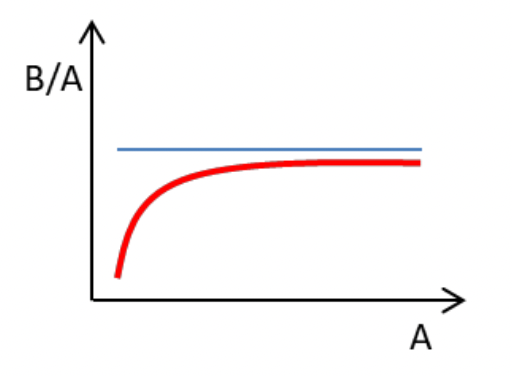
\includegraphics{figs/goccia2}
	%    \caption{This is a margin figure.}
	\label{fig:goccia2}
\end{marginfigure}

Un ulteriore miglioramento può essere ottenuto tenendo presente che i
protoni del nucleo si \emph{respingono elettrostaticamente} diminuendo
quindi il lavoro necessario per separarli dal nucleo stesso.
In effetti
se, per assurdo, si avesse un nucleo composto solo di protoni(senza
neutroni) il lavoro da spendere per mantenerne la configurazione sarebbe
sicuramente maggiore.

Ipotizzando una \emph{distribuzione di protoni uniforme} nel volume
nucleare(ricordiamo essere sferico dall'ipotesi precedente), otteniamo
la seguente espressione del lavoro fatto dalle forze coulombiane
repulsive per separare la carica nucleare
\begin{gather*}
	\delta L = \int _{R}^{\infty} \left( \frac{q \delta q}{4 \pi \epsilon_{0}r^{2}}  \bm{i}_{r} \right)(dr \bm{i}_{r})=
	- \frac{q \delta q}{4 \pi \epsilon_{0}r} \bigg |_{R}^{\infty} =
	- \frac{q \delta q}{4 \pi \epsilon_{0}R}\\
	q = \rho \frac{ 4}{3} \pi R^{3} \qquad \delta q = \rho 4 \pi R^{2} dR\\
	\delta L = \frac{1}{4 \pi \epsilon_{0}R}\left( \rho \frac{ 4}{3}\pi R^{3} \right)(\rho 4 \pi R^{2} dR) = \frac{4 \pi \rho^{2}}{3 \epsilon_{0}}R^{4}dR\\
	L = \int \delta l = \frac{4 \pi \rho^{2}}{15 \epsilon_{0}}R_{0}^{5} \qquad Q = \rho \frac{ 4}{3} \pi R_{0}^{3} = Ze\\
	L = \frac{3}{20 \pi \epsilon_{0}} \frac{Q^{2}}{R_{0}} = \frac{3e^{2}}{20 \pi \epsilon_{0}r_{0}} \frac{Z^{2}}{A^{1/3}}
	\implies L \propto \frac{ Z^{2}}{A^{1/3}}\\
\end{gather*} Ne consegue che la energia di legame nucleare dovrà essere corretta
sottraendo un termine proporzionale a \(Z^{2} / A^{1/3}\) per cui
l'espressione dell'energia di legame acquisirà la forma seguente \[
	B = a_{v}A - a_{s}A^{2/3} - a_{c} \frac{Z^{2}}{A^{1/3}}
\] dove la nuova costante \(a_{c}\) viene detta \textbf{termine
	coulombiano}.
Il termine coulombiano deve chiaramente annullarsi per
\(A=1\)(non c'e interazione elettrostatica) per cui l'unica forma
possibile è \[
	L \propto \frac{Z(Z-1)}{A^{1/3}} \quad
\]
\begin{marginfigure}
	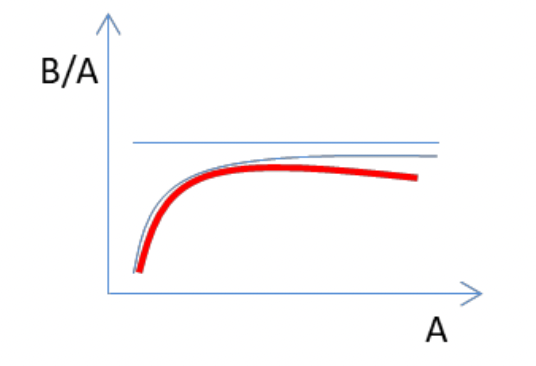
\includegraphics{figs/goccia3}
	%    \caption{This is a margin figure.}
	\label{fig:goccia3}
\end{marginfigure}

L'andamento \(B/A\) risulta ulteriormente migliorato (si tenga presente
che nei nuclei stabili si ha approssimativamente \(Z=A/2\) per cui il
termine coulombiano sottrae un contributo crescente con \(A^{2/3}\)).

Se il modellino fenomenologico costruito finora fosse completo dovremmo
concludere che i nuclei più stabili(\(B= B_{max}\)) sono quelli con
\(Z=0\) ovvero i nuclei di soli neutroni.
Tale fatto è palesemente
contraddetto dai dati sperimentali i quali mostrano che i nuclei stabili
hanno un numero di protoni di poco inferiore a quello dei neutroni (la
differenza tra neutroni e protoni tende a crescere con il numero
atomico).
Il nostro modello -- basato sulla natura a corto raggio della
interazione nucleare -- non offre alcun appiglio per dare un fondamento
fisico a questo stato di cose che potrà essere spiegato solo nel
contesto della meccanica quantistica attraverso il \emph{principio di
	esclusione di Pauli}.
In questa situazione l'unica possibilità è quella
di introdurre un termine `ad hoc' capace di descrivere i dati
sperimentali.

Bisogna quindi fare in modo che il modello ci dica che i nuclei piu
stabili sono quelli con lo stesso numero di protoni e neutroni.
Raggiungiamo l'obiettivo introducendo un nuovo termine del tipo:
\[
	Z \simeq \frac{A}{2} \quad A - 2Z \simeq 0
\]
Ricordando però che con il crescere di \(A, Z\) tende ad essere via
via più piccolo di \(A/2\) (il quoziente protoni/neutroni diminuisce con
\(A\)), tale termine correttivo dovrà seguire una legge inversa ad A
modulata da un qualche esponente.
I dati indicano che la prima potenza è
sufficiente per cui abbiamo la seguente espressione della energia di
legame nucleare
\[
	B = a_{v}A - a_{s}A^{2/3} - a_{c} \frac{Z(Z-1)}{A^{1/3}} - \frac{a_{a}(A-2Z)^{2}}{A}
\]
dove la nuova costante \(a_{a}\) viene detta \textbf{termine di asimmetria}.
Notiamo che la presenza di \(A\) a denominatore è
giustificata osservando l'andamento dei dati sperimentali nel grafico
visto in precedenza:tanto piu \(A\) è grande tanto piu \(B / A\) devia
dalla tangente alla curva(quindi verso il basso).

Per completare il modello è necessario tenere conto di un ulteriore
proprietà dei nuclei.
I dati sperimentali mostrano che tra i 254 nuclei
stabili noti ben 148 sono del tipo \textbf{pari-pari} (un numero pari
sia di protoni che di neutroni), 101 sono del tipo \textbf{pari-dispari}
(un numero pari di protoni ma dispari di neutroni o viceversa) e solo 5
sono del tipo dispari-dispari (vedi tabella).
Similmente, tra i 35
nuclei a lunga vita media si hanno 22 pari-pari, 9 pari-dispari e 4
dispari-dispari.
\begin{marginfigure}
	\centering
	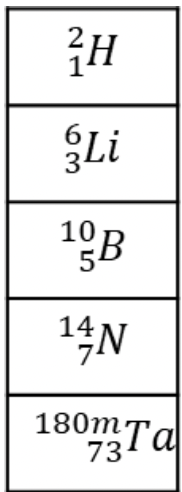
\includegraphics[height = 0.35 \textheight]{figs/goccia4}
	%    \caption{This is a margin figure.}
	\label{fig:goccia4}
\end{marginfigure}
Tali dati sembrano suggerire che per qualche motivo la forza forte tra
nucleoni da luogo a nuclei di maggiore stabilità quando vengono legati
\textbf{numeri pari} di neutroni e protoni, un fatto che trova una sua
diretta evidenza nell'andamento della energia di legame per nucleone
della serie isotopica dello xenon.
Tali dati sembrano suggerire che per qualche motivo la forza forte tra nucleoni da luogo a nuclei di maggiore stabilità quando vengono legati **numeri pari** di neutroni e protoni, un fatto che trova una sua diretta evidenza nell’andamento della energia di legame per nucleone della serie isotopica dello xenon.
\begin{marginfigure}
	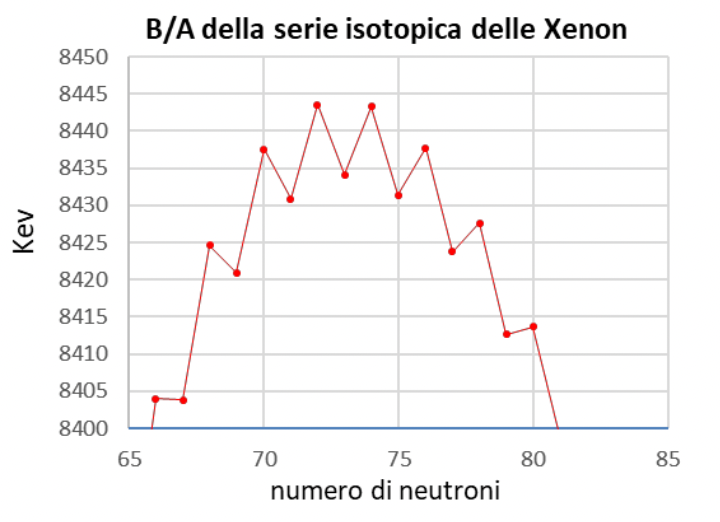
\includegraphics[scale = 1.5]{figs/goccia5}
	%    \caption{This is a margin figure.}
	\label{fig:goccia5}
\end{marginfigure}
Tenendo presente che il nucleo di Xenon ha \(Z=54\) protoni, si può
infatti constatare che gli isotopi con un numero pari di neutroni hanno
una maggiore energia di legame per nucleone.
Per rendere conto di questo
fatto si introduce un nuovo coefficiente detto di \textbf{pairing} \[
	a_{p} \frac{\delta}{A^{3/4}}
\] con \[
	\delta =
	\begin{cases}
		+1    \qquad  \text{pari-pari}       \\
		\ 0  \qquad  \ \ \text{pari-dispari} \\
		-1  \qquad  \text{dispari-dispari}
	\end{cases}
\] Giungiamo così alla seguente espressione complessiva della energia di
legame nucleare detta anche \textbf{formula semiempirica della energia
	di legame nucleare} o \textbf{formula di Weizsacker} della energia di
legame nucleare \begin{equation}
	\boxed{    B = a_{v}A - a_{s}A^{2/3} - a_{c} \frac{Z(Z-1)}{A^{1/3}} - a_{a}\frac{(A-2Z)^{2}}{A} +     a_{p} \frac{\delta}{A^{3/4}}}
\end{equation} Essa dipende da \(5\) parametri il cui valore numerico
viene determinato adattando la formula ai dati sperimentali di\(B/A\).
A
titolo di esempio, una possibile combinazione di valori è la seguente(i
valori sono in \(MeV\)): \[
	a_{v} = 15.5 \quad a_{s} = 16.8 \quad a_{c} = 0.72 \quad a_{a} = 23.0 \quad a_{p} = 34.0
\]

La formula della energia di legame nucleare è utile - come strumento di
calcolo - perchè suggerisce una prima interpretazione del nucleo e delle
forze che lo tengono insieme.

Da essa deduciamo che le forze tra nucleoni devono essere \textbf{molto
	intense} ma a \textbf{short range} (proprietà di saturazione), producono
una distribuzione spaziale tendenzialmente uniforme di nucleoni e
conducono ad una espressione della energia di legame con termini di
volume e superficie in analogia con quanto accade per i liquidi, ragione
che giustifica il nome spesso usato di \textbf{modello nucleare a
	goccia}.

Il modello a gas di fermioni (giustificabile con considerazioni
quantomeccaniche )riesce a rendere conto del termine \(a_{a}\) mentre
fallisce per quello di pairing.
Vedremo che il modello a shell sarà
quello piu preciso.


\section{Richiami di meccanica quantistica}\label{richiami-di-meccanica-quantistica}

\subsection{Osservabili e valori di aspettazione}\label{sec:osservabili-e-valori-di-aspettazione}

I sistemi fisici microscopici in regime non relativistico sono descritti
dalla funzione d'onda \(\psi(\bm{r},t)\) che si assume descriva in modo
completo lo stato fisico della particella, ovvero dica tutto ciò che può
essere detto su di essa.
Il significato fisico della funzione d'onda è
definito dalla ipotesi di Born secondo la quale il \emph{modulo quadrato
	fornisce la densità di probabilità di localizzazione della particella
	nel punto} \(\bm{r}\) al tempo t a seguito della interazione con un
apparato di misura: \[
	| \psi(\bm{r},t)|^{2}dV
\] Tale ipotesi comporta la \textbf{condizione di normalizzazione},
ovvero che l'integrale del modulo quadrato della funzione d'onda sul
volume occupato dal sistema microscopico debba essere pari ad uno, e
stabilisce che in meccanica quantistica la \textbf{grandezza fisica
	osservabile} sia il modulo quadrato della funzione d'onda piuttosto che
la funzione d'onda stessa.

Si assume infine che l'evoluzione temporale della funzione d'onda sia
governata dalla equazione di Schrödinger \[
	i \hslash \frac{\partial}{\partial t} \psi = \hat{H} \psi \qquad \hat{H} = - \frac{\hslash^{2}}{2m} \nabla^{2} + V
\] Come possiamo arrivare al \textbf{valore di aspettazione} di
posizione e quantità di moto?
Calcolo del valore medio della posizione
di una particella.
Nel caso di un' onda piana: \[
	\psi(\bm{r},t) = \psi_{0} e^{ i/\hslash (\bm{p} \cdot \bm{r}-Et) }
\] se \(p\) ed \(E\) fossero sempre definiti avrei che tutte le
posizioni nel piano hanno la stessa probabilità di essere misurate.
Per
cui una misurazione ripetuta potrebbe portare ad un esito diverso della
posizione. \(\implies\)ragionamento in termini
statistici\(\implies\)posso solo conoscere il \textbf{valore medio}
della posizione. \[
	\bm{r} |\psi(\bm{r},t)|^{2}dV \qquad <\bm{r}> = \sum_{i}^{n} \frac{\bm{r}_{i}p_{i}}{\sum_{i}^{n}p_{i}}
\]

\begin{equation}
	<\bm{r}> = \frac{\iiint_{V} \bm{r} |\psi(\bm{r},t)|^{2}dV }{\iiint_{V}|\psi(\bm{r},t)|^{2}dV }
\end{equation} dove il denominatore è unitario dalla condizione di
normalizzazione.
A questo punto si ha, con \(\psi^*\) complesso
coniugato, \[
	<\bm{r}> = \iiint_{V} \psi^*(\bm{r},t)\bm{r}\psi(\bm{r},t)\,dV
\] ovvero la \emph{media delle posizioni corrisponde alla media del
	vettore posizione \(\bm{r}\) pesata dal modulo quadro della funzione
	d'onda.}

Meno immediato è comprendere come calcolare ad esempio la quantità di
moto della particella.
Ragionando ancora una volta in modo euristico
possiamo richiamare le espressioni, scritte nel capitolo precedente, per
una data componente di Fourier della funzione d'onda \[
	- i \hslash \psi(\bm{r},t) = \hat{P} \psi(\bm{r},t) = \bm{p} \psi(\bm{r},t) \qquad
	i \hslash \frac{\partial}{\partial t} \psi(\bm{r},t) = \hat{E}\psi(\bm{r},t)= E\psi(\bm{r},t)
\] Si vede che nel caso in cui la funzione d'onda abbia quantità di moto
ed energia definite (ovvero nel caso in cui la funzione d'onda coincida
con una data componente di Fourier) allora gli operatori a primo membro
estraggono da essa i corrispondenti valori ponendoli nella posizione di
autovalori ovvero di moltiplicatori.
In meccanica quantistica si assume
che tale fatto abbia valida generale:

\begin{quote}
	Se in uno stato quantomeccanico \(\psi\) un osservabile ha un valore
	definito \(o\) allora lo stato \(\psi\) è autostato del corrispondente
	operatore \(O\) con autovalore \(o\)(\(O \psi = o \psi\)).
\end{quote}

Proseguendo nel ragionamento, operando sulla prima delle equazioni
precedenti(prima moltiplicando per \(\psi^{*}\) e poi integrando ambo i
membri) si ha

\begin{gather*}
	- i \hslash \nabla \psi = \bm{p} \psi \implies
	\psi^{*}(-i \hslash \nabla) \psi = \bm{p} \psi^{*}\psi\\
	\iiint_{V} \psi^{*}(-i \hslash \nabla) \psi \, dV = \iiint_{V} \bm{p} \psi^{*}\psi \, dV = \bm{p}\\
\end{gather*} dove si è sfruttata la normalizzazione della funzione d'onda.
Si noti
che tale espressione, valida nel caso di una data componente di Fourier,
è strutturalmente analoga alla posizione media delle posizioni della
particella microscopica (\(33\)) valida invece in generale.
Non è
difficile mostrare che nel caso di un generico pacchetto d'onde il
valore medio della quantità di moto della particella continua ad essere
dato da questo integrale per cui scriveremo \[
	<\bm{p}> = \iiint_{V} \psi^{*}\hat{P}\psi \, dV = \iiint_{V} \psi^{*}(- i \hslash \nabla )\psi \, dV
\] Inoltre, essendo le grandezze fisiche espresse da numeri reali, gli
operatori associati alle variabili dinamiche dovranno essere
\textbf{hermitiani}.

Giungiamo allora a formulare uno degli assiomi della meccanica
quantistica nella seguente forma:

\begin{quote}
	Ad ogni grandezza fisica misurabile \(o\) (osservabile) di un dato
	sistema microscopico, risulta associato un operatore lineare complesso
	hermitiano \(O\).
	Il valore medio delle misure della osservabile \(o\)
	al tempo \(t\) in un certo stato quantomeccanico \(\psi(\bm{r},t)\) è
	dato dal seguente integrale detto valore di aspettazione \[
		\boxed{<o> = \iiint_{V} \psi^{*}(\bm{r},t)\hat{O}\psi(\bm{r},t) \, dV}
	\]
\end{quote}

Quanto detto rende evidente che, dato un sistema quantomeccanico, si
pone il problema fondamentale di individuare le grandezze fisiche
osservabili e di determinare le corrispondenti operatori associati.
La
fisica atomica, ma ancor più la fisica delle particelle, chiariscono che
un criterio generale non esiste e che sia le osservabili che le loro
espressioni operatoriali possono essere trovate solo fondandosi sui dati
sperimentali.\\
Ciò non toglie che si sia verificato che le espressioni operatoriali
delle variabili dinamiche classiche possano essere trovate (sia pure con
alcune limitazioni che per ora tralasciamo) attraverso una procedura,
detta \textbf{principio di corrispondenza} (che applicheremo al caso del
momento angolare), la quale però non può essere applicata nel caso di
variabili dinamiche che non abbiano un corrispondente classico.
In tali
casi l'unica guida rimangono i dati sperimentali ed il percorso può
essere lungo e tortuoso.

\subsection{Definizione ed indefinizione delle osservabili}\label{sec:definizione-ed-indefinizione-delle-osservabili}

Una volta compreso in che modo debbano calcolarsi le variabili dinamiche
di un sistema quantomeccanico è necessario accennare ad un delicato
problema già sullo sfondo di alcune nostre considerazioni.
Riprendiamo
l'esempio dell'onda piana prograssiva visto poco fa. \[
	\psi(\bm{r},t) = \psi_{0}e^{ i/\hslash (\bm{p}\cdot \bm{r}- \omega t)}
\] Con tutta evidenza tale espressione descrive una particella avente
quantità di moto ed energia definite ma posizione spaziale e temporale
completamente \textbf{indefinite}.
Infatti, fissato il tempo, le
superfici equifase dell'onda risultano essere piani perpendicolari al
vettore quantità di moto.
Ciò significa che il modulo quadrato della
funzione d'onda assumerà un valore uniforme sui punti di tali superfici
(in realtà nel caso di una singola componente di Fourier su tutti i
punti dello spazio).
A sua volta ciò significa che la particella potrà
essere localizzata con densità di probabilità uniforme su tutti i punti
della superficie di un piano perpendicolare alla quantità di moto che
equivale ad affermare che la posizione della particella è assolutamente
indefinita.

Un minimo di conoscenza delle proprietà delle onde riconosce in questo
fatto qualcosa di noto poiché sappiamo bene che \emph{una qualunque
	componente di Fourier di un'onda piana possiede vettore d'onda e
	pulsazione definite ma posizione spaziale e temporale assolutamente
	indefinite}.

Sappiamo anche che per avere onde con posizione spaziale e temporale
meglio definite é necessario sovrapporre componenti di Fourier di
diverso vettore d'onda e pulsazione andando a costituire i cosiddetti
pacchetti d'onde.\\
Infine dalla \textbf{fisica classica}\footnote{The general idea is
	present in~\emph{any system where there are plane waves}~A physically
	realizable wave is always in the form of a wave packet which is finite
	in extent. A wave packet is built up by superposing waves with
	definite wave number. By simple Fourier analysis, a highly localized
	packet will require a wide spread of wave vectors, whereas a packet
	with a large spacial extent can be composed of wave numbers quite
	close to a specific value} sappiamo che nei pacchetti d'onde valgono
le cosiddette \textbf{relazioni di indeterminazione} che esprimono
queste proprietà in forma quantitativa approssimata \[
	\Delta k_{x} \Delta x \simeq2 \pi \qquad \Delta \omega \Delta t \simeq2 \pi
\] dove, data una direzione x dello spazio, \(\Delta k_{x}\) e
\(\Delta \omega\) stimano la dispersione del vettore d'onda e della
pulsazione del pacchetto, mentre \(\Delta x\) e \(\Delta t\) ne stimano
la dispersione spaziale e temporale.

\begin{marginfigure}
	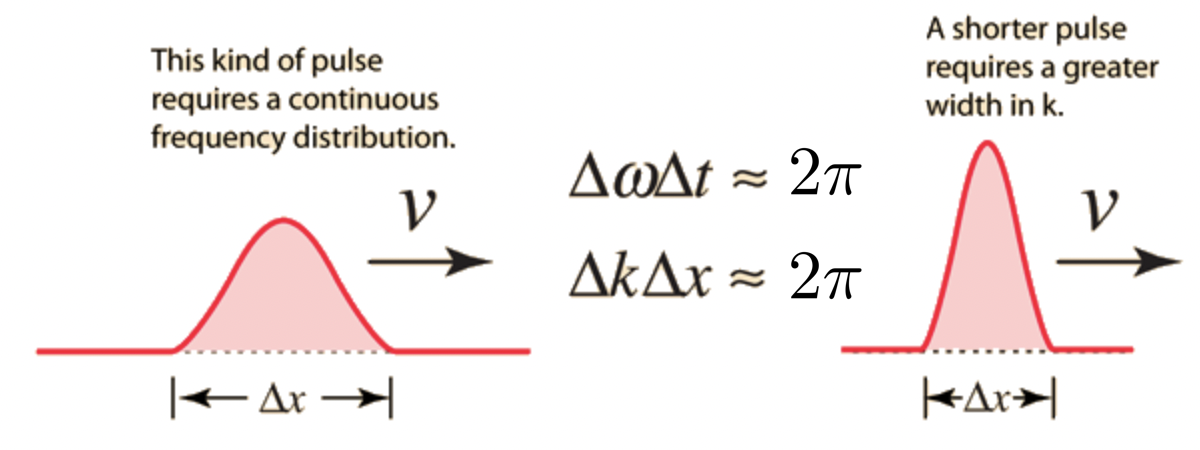
\includegraphics{figs/rel-indet}
	%    \caption{This is a margin figure.}
	\label{fig:rel-indet}
\end{marginfigure}

In generale si può dimostrare che valgono le seguenti relazioni \begin{gather*}
	\Delta k_{x} \Delta x \simeq2 \pi\\
	\Delta k_{y} \Delta y \simeq2 \pi\\
	\Delta k_{z} \Delta z \simeq2 \pi\\
	\Delta \omega \Delta t \simeq2 \pi\\
\end{gather*} Nel caso in cui si abbia un pacchetto d'onde che contenga solo una
componente di Fourier si avrebbe
\(\Delta k_{x} = \Delta k_{y} = \Delta k_{z} = 0\) con una conseguente
indeterminazione sulle posizioni tendente a \(\infty\).

Consideriamo il caso di un'onda piana,di lunghezza d'onda \(\lambda\) e
vettore d'onda \(\bm{k} = k_x \hat{\imath}\), che viene fatta passare
attraverso una fenditura ampia \(d\)(vedi figura).

\begin{marginfigure}
	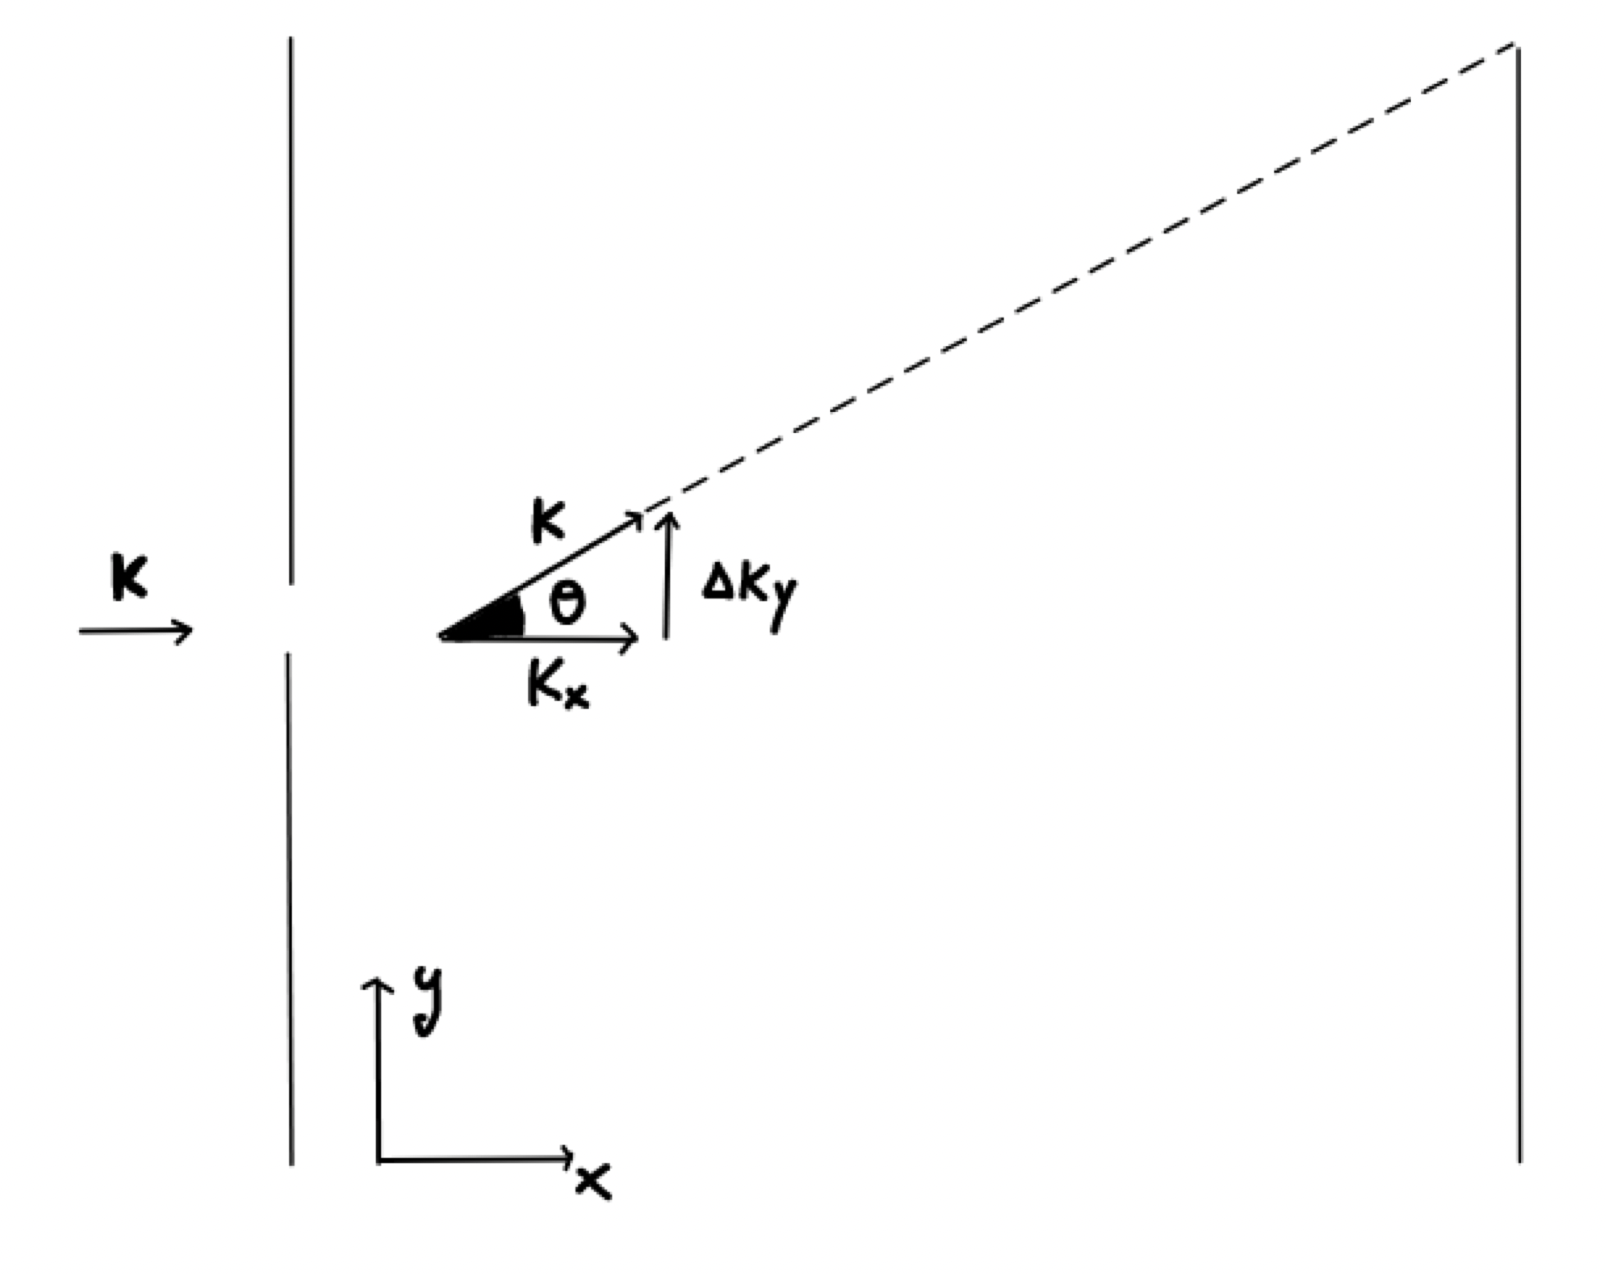
\includegraphics{figs/wave-electron-experiment}
	\caption{This is a margin figure.}
	\label{fig:wave-electron-experiment}
\end{marginfigure}

Il fronte d'onda viene tagliato dalla fenditura stessa:il fronte d'onda
lungo \(y\) ha un'incertezza \(\Delta y = d\).
Dalle relazioni
precedenti so che viene introdotto un errore
\(\Delta k_{y} \simeq\frac{2\pi}{d}\) .
La fenditura ha deviato il
vettore d'onda \(\bm{k}\) ed ora ha una certa angolazione \(\implies\)
il fronte d'onda che si incurva(dal Principio di Huygens-Fresnel).
L'angolo di apertura vale quindi \[
	\theta \simeq\frac{\Delta k_{y}}{k_{x}} \simeq \frac{2\pi}{d  \frac{2\pi}{\lambda}} \simeq\frac{\lambda}{d}
\] In ultima analisi quindi il fronte d'onda viene \textbf{limitato
	spazialmente} e dà luogo al fenomeno della \textbf{diffrazione}.

Vogliamo ora trovare l'analogo delle relazioni di indeterminazione in
\textbf{meccanica quantistica}.
Partiamo dalle relazioni \[
	\bm{p} = \hslash \bm{k} \qquad E = \hslash \omega \qquad p_{x} = \hslash k_{x}
\] e arriviamo a \begin{gather*}
	\Delta p_{x} \Delta x \simeq h\\
	\Delta p_{y} \Delta y \simeq h\\
	\Delta p_{z} \Delta z \simeq h\\
	\Delta E \Delta t \simeq h\\
\end{gather*} relazioni note come \textbf{relazioni di indeterminazione di
	Heisenberg} le quali affermano che

\begin{enumerate}
	\tightlist
	\item
	      se la misura della posizione di un corpuscolo materiale lungo una
	      certa direzione ha una incertezza \(\Delta x\) allora una simultanea
	      misura della quantità di moto lungo la stessa direzione ha una
	      incertezza \(\Delta p_x\) tale che il loro prodotto sia dell'ordine
	      della costante di Plank;
	\item
	      se la misura della posizione temporale di un corpuscolo materiale ha
	      una incertezza \(\Delta t\) allora una simultanea misura della energia
	      ha una incertezza \(\Delta E\) tale che il loro prodotto sia
	      dell'ordine della costante di Planck.
\end{enumerate}

Un analogo quantistico dell'esperimento precedente può consistere
nell'inviare un elettrone con quantità di moto
\(\bm{p} = p_{x} \hat{\imath}\) verso una fenditura di ampiezza \(d\).
Nel
momento in l'elettrone passa in mezzo alla fenditura possiamo
sicuramente dire che la sua posizione assume un qualche valore
\emph{all'interno del range} della fenditura.
Si ha quindi che il passaggio attraverso essa e la conseguente limitazione sulla posizione
della posizione \emph{equivale ad un'operazione di misura} sulla
particella.

\begin{marginfigure}
	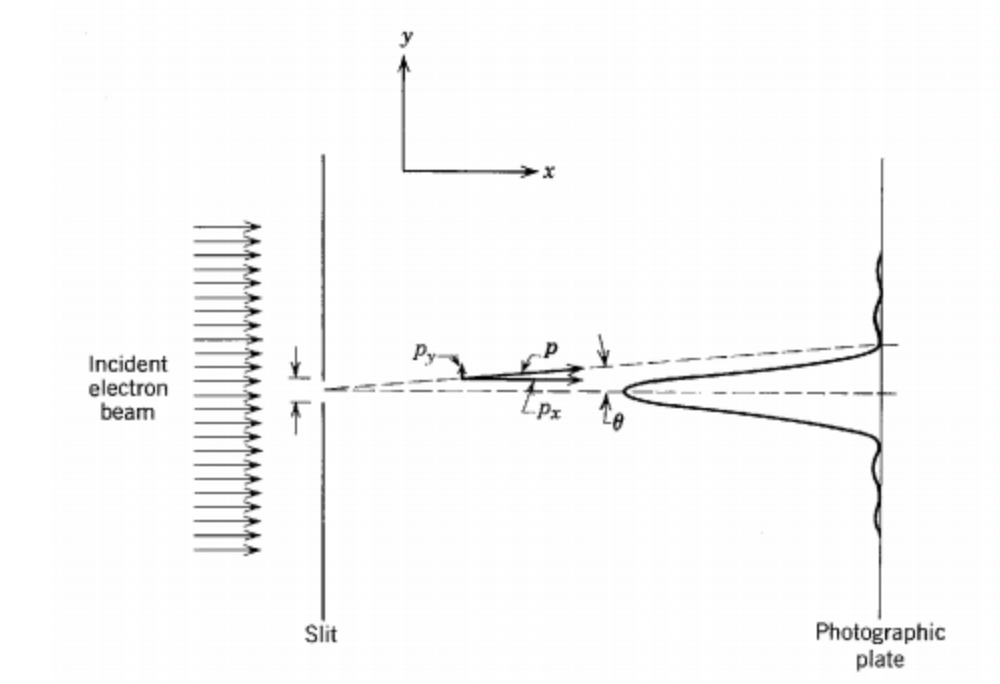
\includegraphics[width = 1.3 \textwidth, height = 1.3 \textheight]{figs/beam-electron-experiment}
	\caption{This is a margin figure.}
	\label{fig:beam-electron-experiment}
\end{marginfigure}

\[
	\Delta y \simeq d \qquad \Delta p_{y} \simeq \frac{h}{d}
\] con angolo di inclinazione
\[
	\theta \simeq \frac{\Delta p_{y}}{p_{x}} \simeq \frac{h}{d \frac{h}{\lambda}} \simeq \frac{\lambda}{d}
\]

L'incompatibilità tra le variabili dinamiche di un sistema
quantomeccanico è espressa in forma precisa da un fondamentale teorema
della meccanica quantistica il quale stabilisce che

\begin{quote}
	Il prodotto delle deviazioni standard delle misure di due grandezze
	fisiche \(a\) e \(b\) in uno stato \(\psi\) è limitato inferiormente dal
	valore di aspettazione del commutatore dei loro operatori diviso il
	fattore \(2i\)
	\begin{equation}
		\sigma_{a} \sigma_{b} \geq \iiint_{V} \psi^{*}(\bm{r},t) \frac{\hat{A}\hat{B} -\hat{B}\hat{A}}{2i} \psi(\bm{r},t) \, dV
	\end{equation}
\end{quote}

A titolo di esempio possiamo considerare proprio le variabili dinamiche
di posizione e quantità di moto\[
\] a = p\_\{x\} \qquad b = x \$\$

con corrispondente operatori \[
	- i \hslash \frac{\partial}{\partial x} \qquad x
\] e calcolarne il commutatore
\[
	\hat{X}\hat{P}_{x} - \hat{P}_{x}\hat{X}
\] per cui calcoliamo i due termini \begin{gather*}
	\hat{X}\hat{P}_{x} \psi = x \left(  - i \hslash \frac{\partial}{\partial x} \right) \psi = - i \hslash x \frac{\partial}{\partial x}\psi\\
	\hat{P}_{x}(\hat{X} \psi) = \left( - i \hslash \frac{\partial}{\partial x} \right)(x \psi)  = - i \hslash \left( \psi - x \frac{\partial}{\partial x} \psi \right) = - i \hslash \psi - i \hslash x \frac{\partial}{\partial x} \psi\\
\end{gather*} ed otteniamo \[
	(\hat{X}\hat{P}_{x} - \hat{P}_{x}\hat{X}) \psi = - i \hslash x \frac{\partial}{\partial x}\psi - \left[ - i \hslash \psi - i \hslash x \frac{\partial}{\partial x} \psi \right] = i \hslash \psi
\] da cui il valore del commutatore \[
	\hat{X}\hat{P}_{x} - \hat{P}_{x}\hat{X} = i \hslash  \hat{1}
\] che sostituito nella \((34)\) fornisce
\begin{gather*}
	\sigma_{x} \sigma_{p_{x}} \geq \iiint_{V} \psi^{*}(\bm{r},t) \frac{\hat{X}\hat{P}_{x} - \hat{P}_{x}\hat{X}}{2 i } \psi(\bm{r},t) \, dV =
	\iiint_{V} \psi^{*}(\bm{r},t) \frac{i \hslash  \hat{1}}{2i}\psi(\bm{r},t) \, dV\\
	\sigma_{x}\sigma_{p_{x}} \geq \frac{\hslash}{2}\\
\end{gather*} che esprime in forma rigorosa il principio di indeterminazione per le
misure della posizione e quantità di moto.

\subsection{Momento angolare orbitale}\label{sec:momento-angolare-orbitale}

Il momento angolare orbitale è un ottimo esempio per comprendere come si
possa utilizzare il \emph{principio di corrispondenza} per costruire
l'operatore quantomeccanico di una variabile dinamica a partire dalla
sua espressione classica
\[
	\bm{l}  = \bm{r} \wedge \bm{p}
\]
L'idea è quella di ottenere l'espressione quantomeccanica
dell'operatore associato attraverso la sostituzione diretta delle
variabili classiche con i corrispondenti operatori quantistici.
Richiamando allora gli operatori posizione e quantità di moto, otteniamo
la seguente espressione della terna ordinata di operatori che
costituiscono \textbf{l'operatore momento della quantità di moto}
\[
	\hat{L} = \hat{r} \wedge \hat{P}=\bm{r} \wedge (- i \hslash \nabla) = - i \hslash \ \bm{r} \wedge \nabla
\]
la quale, nel sistema di coordinate cartesiano, assume la seguente forma
\[
	\hat{L} = (\hat{L}_{x}, \hat{L}_{y}, \hat{L}_{z}) = - i \hslash \left( y \frac{\partial}{\partial z} - z \frac{\partial}{\partial y},z \frac{\partial}{\partial x}-x \frac{\partial}{\partial z}, x \frac{\partial}{\partial y} - y \frac{\partial}{\partial x} \right)
\] Dato che le proprietà generali di un operatore possono essere
studiate attraverso le sue relazioni di commutazione, utilizziamo la
foma cartesiana esplicita per calcolare i commutari della terna di
operatori.
Si ottiene facilmente
\[
	[\hat{L}_{x},\hat{L}_{y}] = i \hslash  \hat{L}_{z} \quad
	[\hat{L}_{z},\hat{L}_{x}] = i \hslash  \hat{L}_{y} \quad
	[\hat{L}_{y},\hat{L}_{z}] = i \hslash  \hat{L}_{x}
\]
Verifichiamo allora che uno stato quantomeccanico non ammette valori
definiti del momento della quantità di moto lungo \(x, y\) e \(z\)
poiché la proiezione lungo \(x\) è incompatibile con quella lungo \(y\),
quella lungo z con quella lungo \(x\) e quella lungo \(y\) con quella
lungo \(z\).
Ciò significa che \emph{in uno stato quantomeccanico il
	momento angolare può assumere valori definiti lungo una sola direzione}
che solitamente si assume come asse \(z\).

Consideriamo ora l'operatore \textbf{modulo quadrato del momento
	angolare} \[
	\hat{L}^{2} = \hat{L}_{x}^{2} + \hat{L}_{y}^{2} + \hat{L}_{z}^{2}
\] Sempre con calcolo diretto si ottengono facilmente i seguenti
commutatori \[
	\left[ \hat{L}^{2},\hat{L}_{x}\right] = \left[ \hat{L}^{2},\hat{L}_{y}\right] = \left[ \hat{L}^{2},\hat{L}_{z}\right] = 0
\]
\begin{marginfigure}
	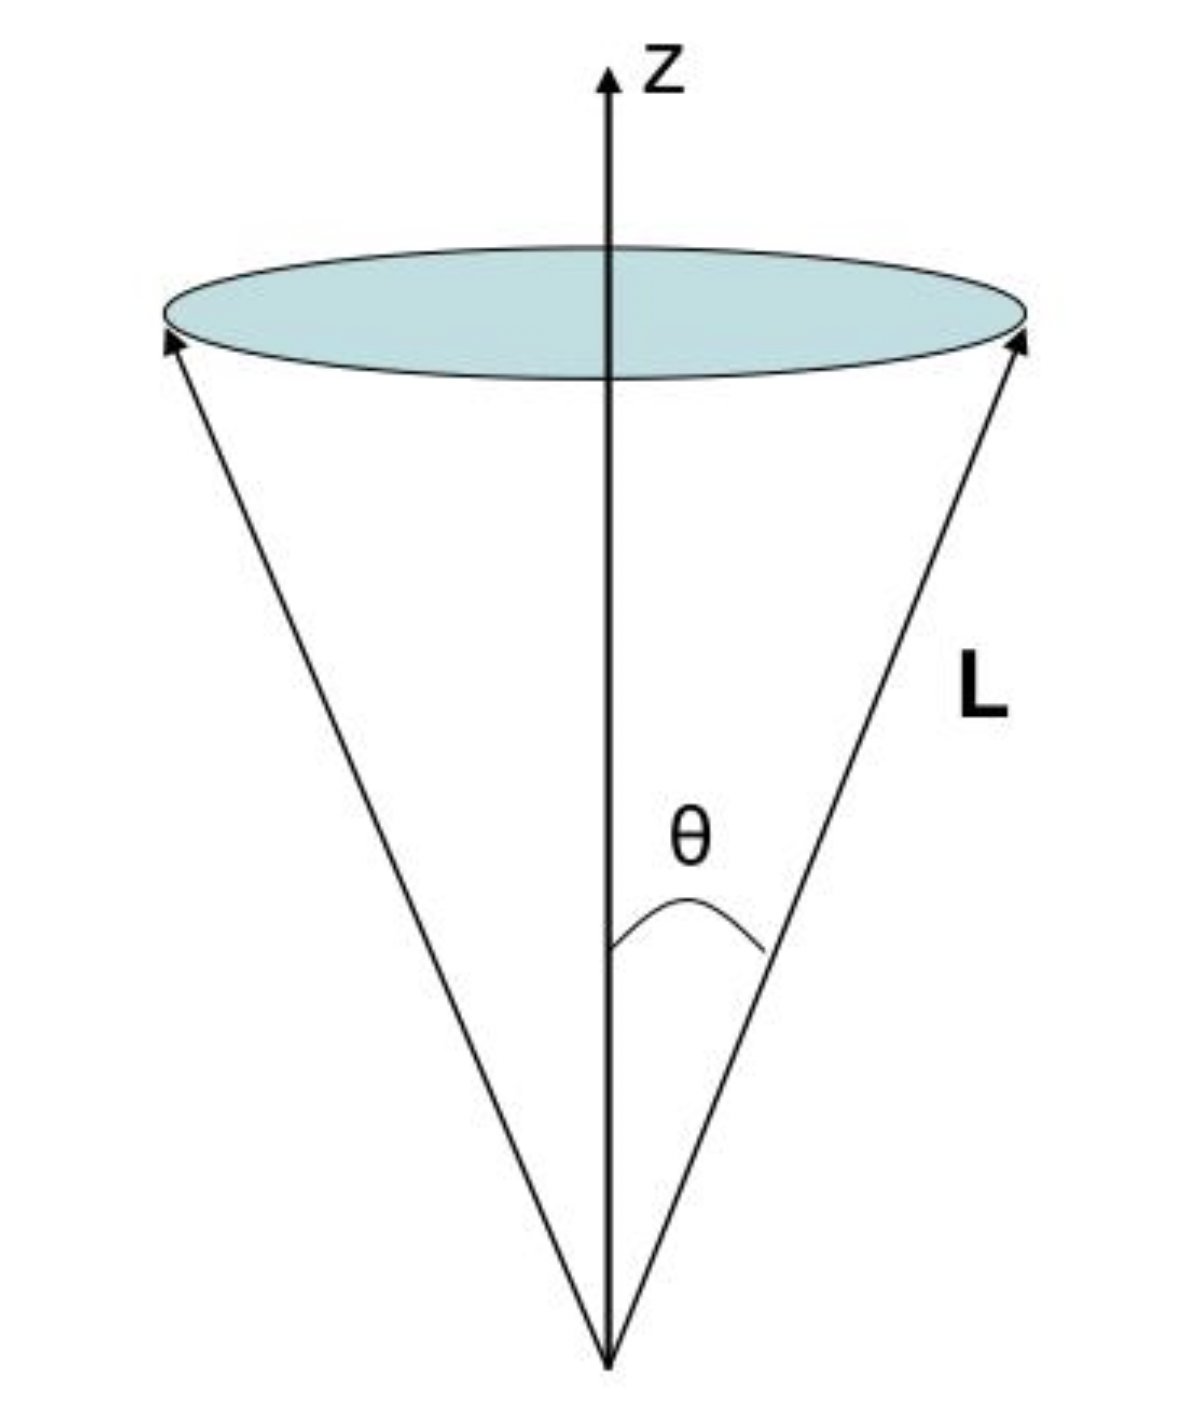
\includegraphics{figs/ang-mom-cone}
	\caption{Il set dei possibili valori di $\hat{L_x}$ e $\hat{L_y}$ descrive un cono attorno ad $\hat{L}_z$}
	\label{fig:ang-mom-cone}
\end{marginfigure}


Dalle relazioni di commutazioni scritte, concludiamo allora che
\textbf{uno stato quantomeccanico ammette valori definiti del quadrato
	del momento angolare e della sua componente lungo \(z\)}.

Giunti a questo punto si pone il problema di stabilire quali siano i
valori definiti del quadrato del momento angolare e della sua componente
lungo z e quali siano le espressioni della funzione d'onda dei
corrispondenti stati quantomeccanici.
Per rispondere a queste domande
occorre risolvere le equazioni agli autovalori degli operatori.
In
particolare, gli \textbf{autovalori forniranno i possibili valori del
	quadrato del momento angolare e della sua terza componente}, mentre le
corrispondenti \textbf{autofunzioni} forniranno le espressioni delle
\textbf{funzioni d'onda} degli stati quantomeccanici: \begin{gather*}
	\hat{L}^{2}\psi = \lambda \psi\\
	< \hat{L}^{2}> = \iiint_{V} \psi^{*} \hat{L}^{2}\psi \, dV = \lambda \iiint_{V} \psi \psi^{*} \, dV = \lambda\\
	\hat{L}^{2} \psi = \lambda' \psi \qquad  \hat{L}_{z} \psi = \lambda'' \psi\\
\end{gather*} Sviluppando il conto si ha \begin{gather*}
	\hat{L}^{2}\psi = l(l+1) \hslash^{2} \psi \qquad l = 0,1,2, \dots , n\\
	\hat{L}_{z} \psi = m \hslash \psi \qquad m = -l,-l + 1, \dots ,l-1, l\\
\end{gather*} Siamo difronte ad un operatore \textbf{quantizzato} ovvero che può
assumere valori \textbf{discreti}:i numeri interi l ed m descrivono
compiutamente lo stato quantomeccanico e vengono detti numeri quantici
del momento angolare.\\
\begin{marginfigure}
	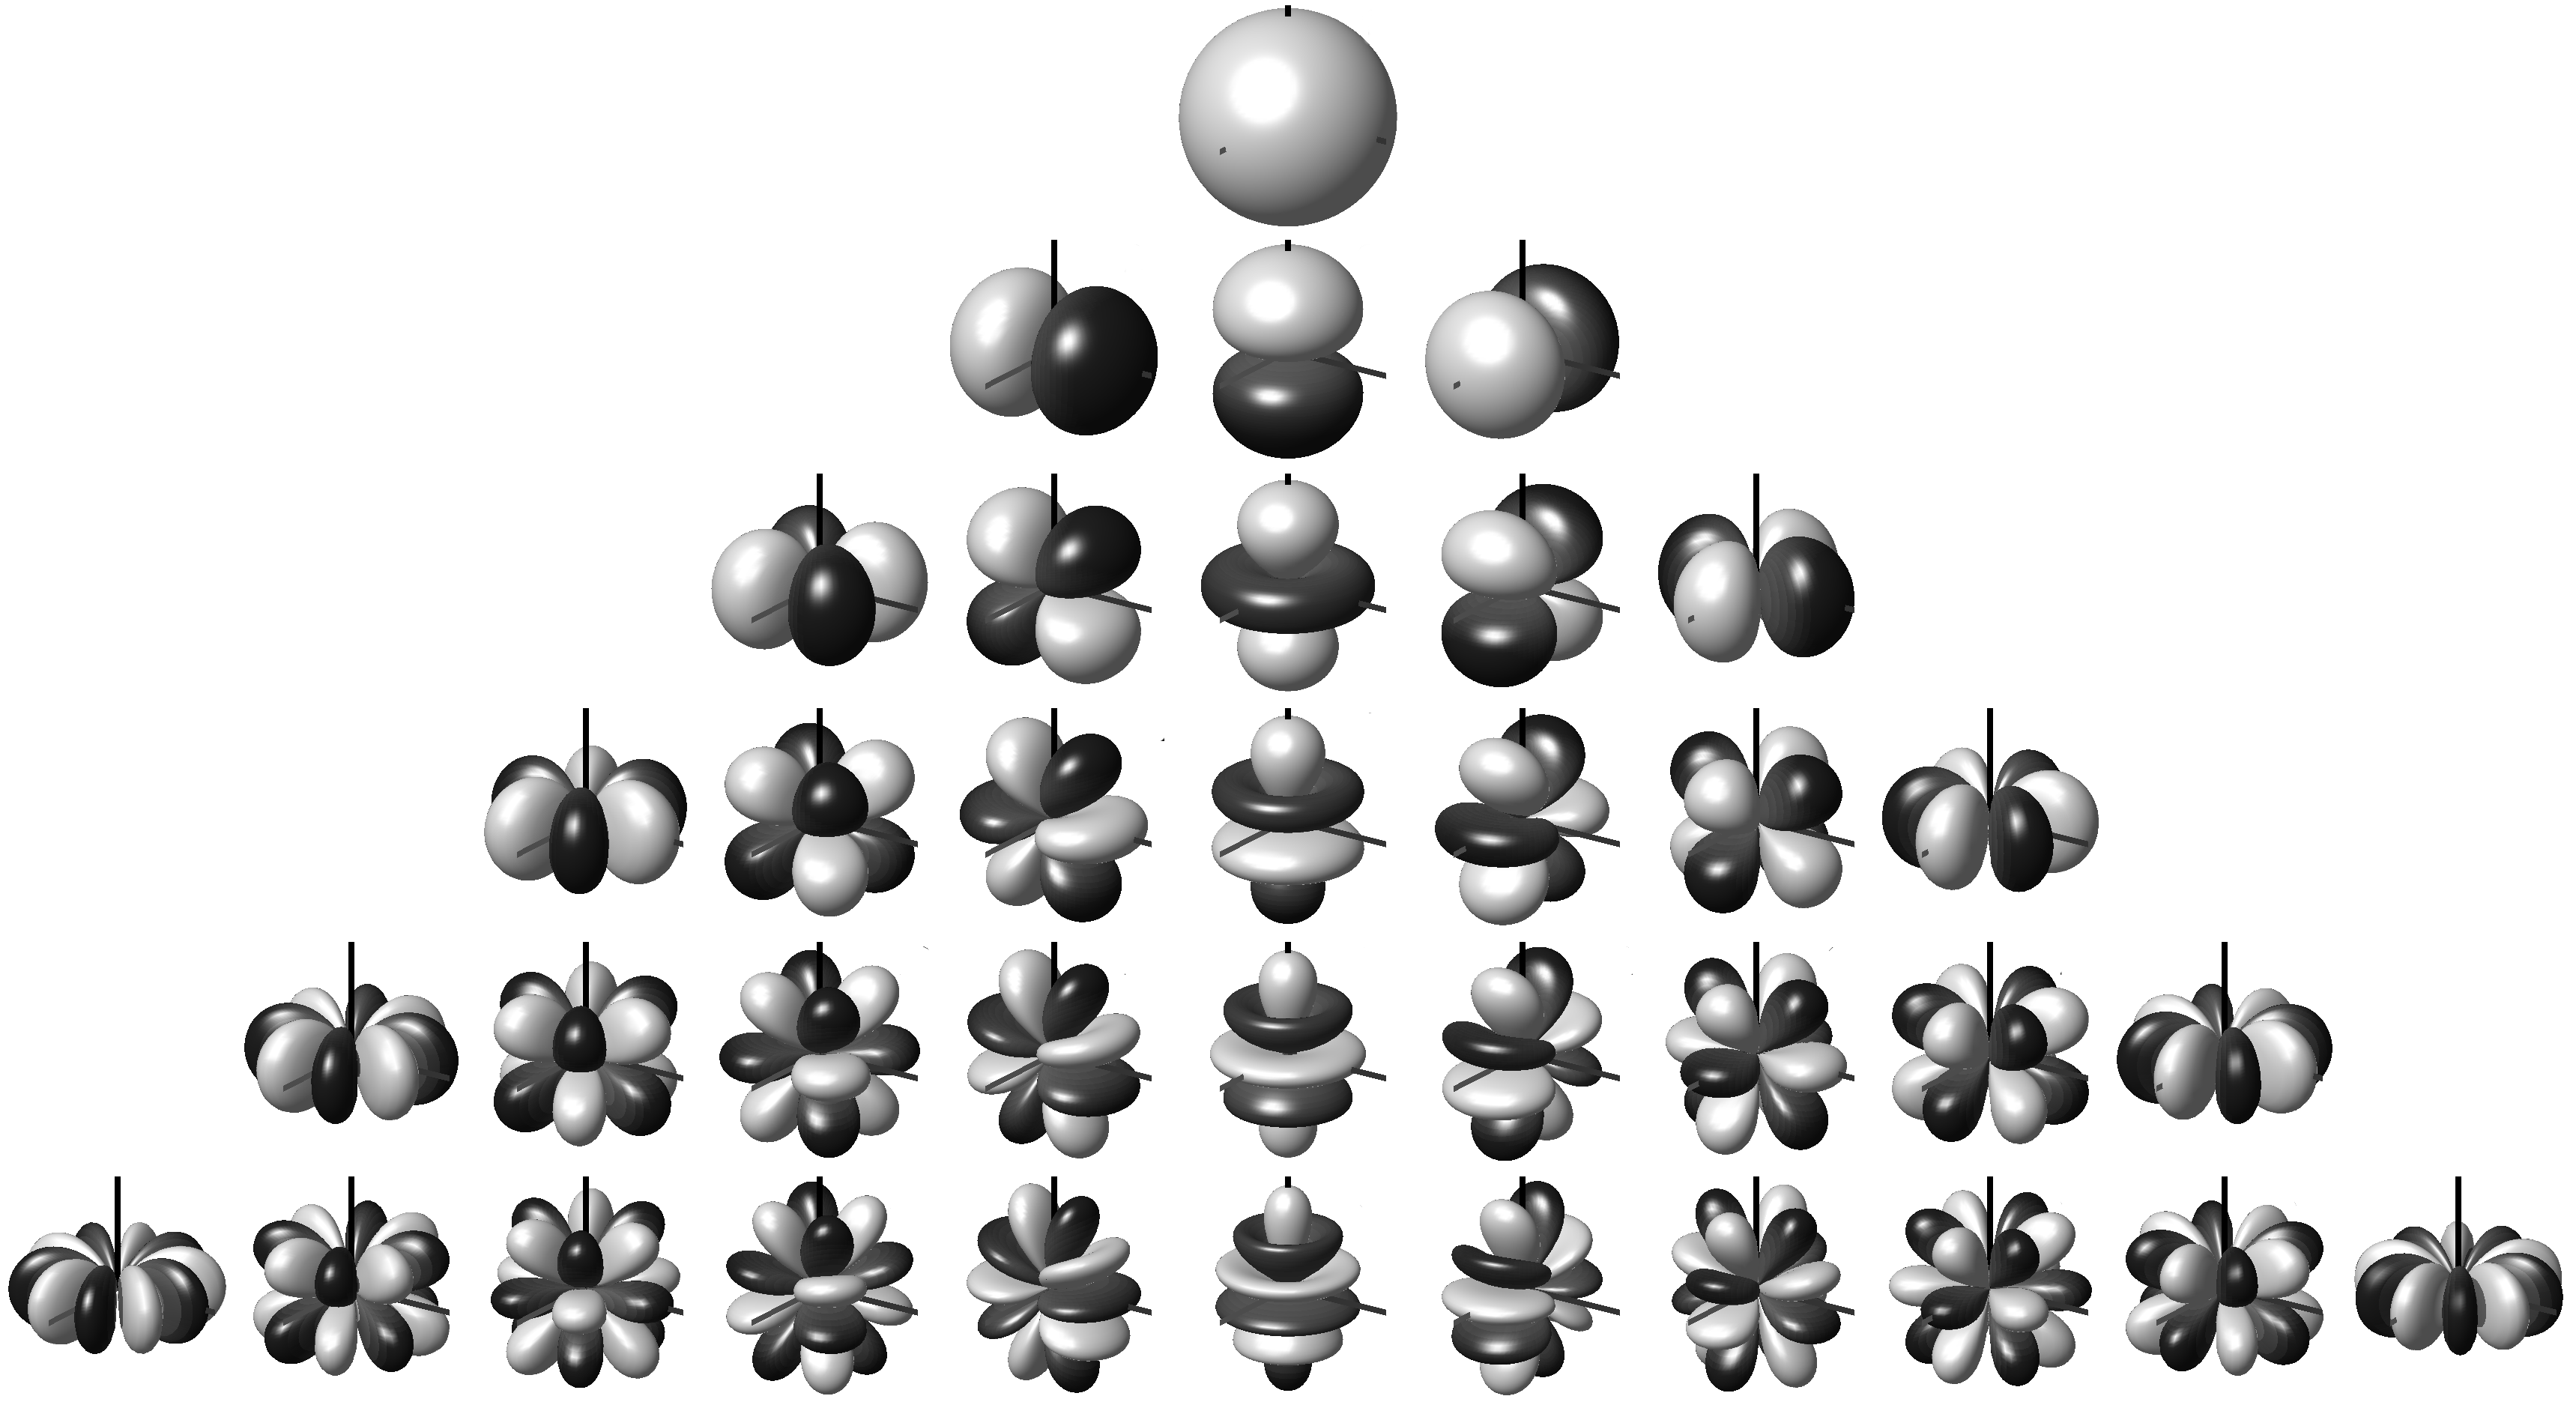
\includegraphics{figs/spherical-harmonics}
	\caption{Rappresentazione grafica delle prime armoniche sferiche.}
	\label{fig:spherical-harmonics}
\end{marginfigure}
In particolare le coppie di valori l ed m individuano spefiche funzioni
d'onda \(\psi_{l,m}(\theta,\phi)\) dette \textbf{armoniche sferiche}.
This peculiar set of functions comes out in the classical theory as well
when considering the modes of oscillation of a 2-dimensional membrane.

I possibili valori del quadrato del momento angolare sono dati dalla
successione discreta \(l(l+1) \hslash^{2}\) dove \(l=0,1,2 \dots\)
mentre i possibili valori del momento angolare lungo z sono dati dalla
successione discreta \(m \hslash\) dove
\(m = -l, -l + 1, \dots, l-1, l\) ovvero da una sequenza di \(2l+1\)
valori interi dipendente da \(l\).

\subsection{Momento angolare intrinseco o spin}\label{sec:momento-angolare-intrinseco-o-spin}

Nella meccanica classica i corpi materiali puntiformi possiedono al più
solo momento angolare orbitale mentre quelli estesi possono essere
portatori anche di un momento angolare intrinseco (spin).
Scegliendo il
polo di riduzione coincidente con il centro di massa del corpo
materiale, il momento angolare orbitale si annulla e l'unico momento
angolare residuo del corpo esteso è quello intrinseco che si manifesta
come rotazione del corpo stesso attorno ad un asse baricentrico.

Date queste premesse, ci si può domandare se anche le particelle
microscopiche possiedano un momento angolare intrinseco (spin) in
aggiunta al momento angolare orbitale.
I fatti sperimentali mostrano che
la risposta è affermativa e che il momento angolare intrinseco o spin
deve essere introdotto anche nel caso delle particelle microscopiche.
Vi
sono però delle sostanziali differenze

\begin{itemize}
	\tightlist
	\item
	      \textbf{meccanica classica}: un momento angolare intrinseco o residuo
	      può esistere solo per i \emph{corpi estesi} (non puntiformi) e questo
	      si interpreta come la somma dei momenti angolari orbitali di tutte le
	      parti che lo compongono;
	\item
	      \textbf{meccanica quantistica}: un momento angolare intrinseco o di
	      spin può esistere anche per le particelle puntiformi e come tale non è
	      riducibile in nessun modo a somme di momenti angolari orbitali delle
	      parti del sistema;
	\item
	      \textbf{meccanica classica}: il modulo del momento angolare intrinseco
	      può assumere con \emph{continuità qualunque valore}, ha un carattere
	      estrinseco e descrive essenzialmente lo stato cinematico di rotazione
	      del sistema rispetto ad un prefissato riferimento;
	\item
	      \textbf{meccanica quantistica}: il modulo del momento angolare
	      intrinseco può assumere un solo valore \emph{fisso} ed
	      \emph{immutabile}.
	      A seguito di tale invariabilità perde il suo
	      carattere estrinseco di natura cinematica ed assume - al pari della
	      massa e delle cariche interne del corpuscolo - lo status di grandezza
	      fisica intrinseca preposta alla descrizione di una nuova proprietà
	      statica della particella.
\end{itemize}

Per questi ed altri motivi possiamo affermare che \emph{lo spin è una
	variabile dinamica essenziamente quantistica} senza una diretta
corrispondenza classica.

Pauli pensò che fosse necessario introdurre una \textbf{terna di
	operatori di spin} \[
	S_{x} \qquad S_{y} \qquad S_{z}
\] soddisfacenti le regole di commutazione `tipo momento angolare' \[
	[ S_{x},S_{y}] = i \hslash S_{z} \qquad  [ S_{y},S_{z}] = i \hslash S_{x} \qquad   [ S_{z},S_{x}] = i \hslash S_{y}
\] ed operano sullo \textbf{spazio degli stati di spin}, uno `spazio
interno' diverso da quello su cui operano gli operatori del momento
angolare orbitale (lo spin è dunque un nuovo grado di libertà del
sistema microscopico).

In analogia con il caso del momento della quantità di moto, le regole di
commutazione appena scritte implicano che \textbf{uno stato
	quantomeccanico ammette valori definiti del modulo quadrato dello spin e
	e della sua terza componente}.

In particolare, risolta l'equazione agli autovalori degli operatori
quadrato del momento angolare di spin e della sua terza componente si
può ottenere l'insieme degli autovalori e delle autofunzioni: \begin{gather*}
	\hat{S}^{2} \eta_{s,s_{z}} = s (s+1) \hslash^{2} \eta_{s,s_{z}} \qquad s = 0, \frac{1}{2}, 1, \frac{3}{2}, \dots\\
	\hat{S}_{z} \eta_{s,s_{z}} = s_{z} \hslash \eta_{s,s_{z}} \qquad s_{z} = -s, -s+1, \dots , s-1, s\\
\end{gather*} dove \(s_{z}\) compie salti unitari tra un valore di \(s\) e il
seguente.
I possibili valori del quadrato del momento angolare di spin
sono dati dalla \(s(s+1)\hslash^{2}\).
Per ciascuno di questi, i
possibili valori del momento angolare di spin lungo \(z\) sono dati
dalla successione discreta di \(2s+1\) valori \(s_{z} \hslash\).
I
numeri \(s\) e \(s_{z}\) descrivono compiutamente lo stato
quantomeccanico e sono detti numeri quantici dello spin.
Essi
individuano specifici vettori \(\eta_{s,s_{z}}\) nello spazio degli spin
e dato che, fissato un certo \(s\) si hanno \(2s+1\) diversi valori di
\(s_{z}\) che individuano \(2s+1\) vettori linearmente indipendenti (e
normalizzati) nello spazio degli spin, ne deriva che \textbf{lo spazio
	dello spin di valore s è uno `spazio interno' complesso di \(2s+1\)
	dimensioni}.

Esempio: - Se \(s = \frac{1}{2}\) allora
\(s_{z} = - \frac{1}{2} , \frac{1}{2}\) ,
\(\eta_{\frac{1}{2},- \frac{1}{2}}, \eta_{\frac{1}{2}, \frac{1}{2}}\) -
Se \(s = 1\) allora \(s_{z} = -1,0,1\) ,
\(\eta_{1,1},\eta_{\frac{1}{2}, \frac{1}{2}}\) - Se \(s = 0\) allora
\(s_{z} = 0\) , \(\eta_{0,0}\) e si dice che la particella non ha spin

Da quanto detto consegue che lo stato quantomeccanico di una particella
microscopica di spin s dovrà essere rappresentato nello \emph{spazio
	prodotto} dello spazio degli stati quantomeccanici `ordinari' già visto,
con lo spazio degli stati di spin, ovvero dalla funzione d'onda `estesa'
\[
	\xi(\bm{r},t) =   \psi(\bm{r},t) \eta_{s,s_{z}}
\] dove \(\eta\) è il vettore di spin.

(È utile sta cosa?)L'analogo classico piu vicino all'onda piana,con
\(\eta_{\frac{1}{2}, \frac{1}{2}}\) ampiezza spinoriale, \[
	\eta_{\frac{1}{2}, \frac{1}{2}} \psi_{0}e^{ i/\hslash (\bm{p}\cdot \bm{r} - Et)}
\] è un'onda piana di campo elettrico \[
	\bm{E}_{0} \sin(\bm{k}\cdot \bm{r} - \omega t)
\]

E' importante sottolineare che l'introduzione di un apposito `spazio
complesso' per la descrizione degli stati di spin delle particelle
microscopiche costituisce un precedente teorico di grande rilevanza.
Essa infatti suggerisce che eventuali gradi di libertà interni delle
particelle richiesti dalla analisi dei dati sperimentali possano essere
descritti in ambito quantomeccanico semplicemente introducendo spazi
vettoriali complessi addizionali dotati della giusta dimensionalità.

\subsection{La somma dei momenti angolari}\label{sec:somma-dei-momenti-angolari}

Sia nei sistemi classici che quantomeccanici accade di dovere calcolare
il momento angolare di un sistema formato da due sottosistemi aventi
ciascuno un dato momento angolare, come si deve fare?

\begin{itemize}
	\tightlist
	\item
	      \emph{Fisica classica}: ai momenti angolari sono associati vettori,
	      pertanto al momento angolare del sistema complessivo si associa la
	      somma vettoriale dei momenti angolari dei due sottosistemi.
	      Dati
	      allora i momenti angolari \(\bm{J}_{1}\) e \(\bm{J}_{2}\) dei due
	      sottosistemi, il momento angolare del sistema complessivo sarà dato
	      dalla somma vettoriale \(\bm{J} = \bm{J}_{1}+ \bm{J}_{2}\) calcolata
	      con la regola del parallelogramma e dipendente da moduli direzioni e
	      versi relativi dei vettori sommati.
	      In particolare, il modulo di tale
	      momento angolare assumerà la seguente serie continua di valori \[
		      \bm{J} = \bm{J_{1}} + \bm{J_{2}} \qquad | |\bm{J_{1}}| - |\bm{J}_{2}| | \leq | \bm{J}| \leq|\bm{J}_{1} | | + | \bm{J}_{2} | |
	      \]
	\item
	      \emph{Meccanica quantistica}: ai momenti angolari sono associati
	      operatori, al momento angolare del sistema complessivo si associata
	      allora la somma operatoriale degli operatori momento angolare dei due
	      sottosistemi.
	      Dati allora gli operatori momento angolare
	      \(\hat{J}_{1}\) e \(\hat{J}_{2}\) dei due sottosistemi, l'operatore
	      momento angolare del sistema complessivo sarà dato dalla somma
	      operatoriale \(\hat{J} = \hat{J}_{1}+ \hat{J}_{2}\).
	      In accordo con le
	      regole generali della meccanica quantistica, si pone allora il
	      problema di determinare autovalori e autostati di tale operatore somma
	      dei momenti angolari.
\end{itemize}

In relazione a questo problema, è semplice mostrare con prova diretta
che se gli operatori \(\hat{J}_{1}\) e \(\hat{J}_{2}\) soddisfano le
relazioni di commutazione viste in precedenza allora anche l'operatore
\(\hat{J} = \hat{J}_{1}+ \hat{J}_{2}\) soddisferà relazioni di
commutazione dello stesso tipo.
Ciò significa che gli operatori
\(J^{2} = (J_{1} + \hat{J}_{2})^{2}\) e
\(\hat{J}_{z} = \hat{J_{1z}} + \hat{J_{2z}}\) avranno in generale i
seguenti autovalori \begin{gather*}
	j(j+1) \hslash^{2} \qquad j = 0, \frac{1}{2}, 1, \frac{3}{2}\\
	m \hslash  \qquad m = -j , -j +1, \dots , j-1, j\\
\end{gather*} Sulla base di considerazioni generali non è possibile dire di più,
per cui risulta necessario citare i risultati del teorema della somma
dei momenti angolari in meccanica quantistica.

Dati allora due stati quantomeccanici con momento angolare definito
\(\phi_{j_{1},m_{1}}\)e \(\phi_{j_{2},m_{2}}\) autostati degli operatori
\(\hat{J}_{1},\hat{J}_{1z}\) e \(\hat{J}_{2}, \hat{J}_{2z}\) si ha \begin{gather*}
	\hat{J}_{1}^{2} \ \phi_{j_{1},m_{1}}(\bm{r}) = j_{1}(j_{1}+1) \hslash \ \phi_{j_{1},m_{1}}(\bm{r}) \qquad j_{1} = 0, \frac{1}{2}, 1, \frac{3}{2}\\
	\hat{J}_{1z} \ \phi_{j_{1},m_{1}}(\bm{r}) = m \hslash \ \phi_{j_{1},m_{1}}(\bm{r})  \qquad m_{1} = -j_{1} , -j_{1} +1, \dots , j_{1}-1, j_{1}\\
	\hat{J}_{2}^{2} \ \phi_{j_{2},m_{2}}(\bm{r}) = j_{2}(j_{2}+1) \hslash \ \phi_{j_{2},m_{2}}(\bm{r}) \qquad j_{2} = 0, \frac{1}{2}, 1, \frac{3}{2}\\
	\hat{J}_{2z} \ \phi_{j_{2},m_{2}}(\bm{r}) = m \hslash \ \phi_{j_{2},m_{2}}(\bm{r})  \qquad m_{2} = -j_{2} , -j_{2} +1, \dots , j_{2}-1, j_{2}\\
\end{gather*} Lo stato quantomeccanico complessivo \(\phi_{j,m}\) è autostato degli
operatori \(J^{2} = (J_{1} + \hat{J}_{2})^{2}\) e
\(\hat{J}_{z} = \hat{J_{1z}} + \hat{J_{2z}}\) dove i loro numeri
quantici\(j\) ed \(m\) soddisfano le seguenti relazioni \begin{gather*}
	\hat{J}^{2} \ \phi_{j,m}(\bm{r}) = j(j+1) \hslash \ \phi_{j,m}(\bm{r}) \qquad | j_{1} - j_{2}|<j<|j_{1}+j_{2}|\\
	\hat{J}_{z} \ \phi_{j,m}(\bm{r}) = m \hslash \ \phi_{j,m}(\bm{r})  \qquad m = m_{1}+m_{2}\\
\end{gather*}

\emph{Esercizio didattico - Spazio di spinori 2 dimensionale}.
Consideriamo uno spazio di spinori identificato da \[
	s = \frac{1}{2} \qquad s_{z} = - \frac{1}{2} , \frac{1}{2}
\] per cui si hanno gli spinori \[
	\xi_{\frac{1}{2}, \frac{1}{2}} \qquad \xi_{- \frac{1}{2}, \frac{1}{2}}
\] Per quanto riguarda gli operatori di spin si ha \[
	\hat{S}^{2} \xi_{\frac{1}{2}, \pm \frac{1}{2}} = \frac{3}{4} \hslash^{2} \xi_{\frac{1}{2}, \pm \frac{1}{2}}
\] e \[
	\hat{S}_{z} \xi_{\frac{1}{2}, \frac{1}{2}} = \frac{1}{2} \hslash \xi_{\frac{1}{2}, \frac{1}{2}} \qquad
	\hat{S}_{z} \xi_{\frac{1}{2}, - \frac{1}{2}} = - \frac{1}{2} \hslash \xi_{\frac{1}{2}, -\frac{1}{2}}
\] Lo spazio è chiaramente bidimensionale dove le direzioni sono
identificate dai 2 spinori: {[}qui disegno di lato {]}

Nel momento in cui si utilizza uno spazio astratto per rappresentare lo
spin è necessario che valga la condizione della sovrapposizione di stati
che giustifica la spazializzazione dello spin.
A livello classico tale
richiesta in uno spazio ordinario sarebbe quella che tutte le posizioni
intermedie fossero accessibili.

In ogni caso siamo interessati solamente agli stati normalizzati, e
dunque non è fondamentale operare in tutto lo spazio, bensì possiamo
restringerci alla sfera unitaria.

Per dare una forma piu semplice e concreta agli spinori, eseguo la
seguente identificazione \[
	\xi_{\frac{1}{2}, \frac{1}{2}} =
	\begin{pmatrix}
		1 \\ 0
	\end{pmatrix} \qquad
	\xi_{\frac{1}{2}, - \frac{1}{2}} =
	\begin{pmatrix}
		0 \\ 1
	\end{pmatrix}
\] Gli operatori \(\hat{S}\) assumeranno forma matriciale in tale
rappresentazione \[
	S_{x,y,z} =
	\begin{pmatrix}
		\alpha & \alpha \\
		\alpha & \alpha
	\end{pmatrix}
\] Dovendo rispettare la condizione che \(S\) sia \emph{autoaggiunta} la
costruiamo come \[
	S_{x,y,z} =
	\begin{pmatrix}
		a      & b - ic \\
		b + ic & d
	\end{pmatrix}
\] Volendo però stare in totale generalità scriveremo

\begin{align*}
	S & =
	\begin{pmatrix}
		a + d & b-ic \\
		b+ic  & a-d
	\end{pmatrix} \\
	  & =
	a
	\begin{pmatrix}
		1 & 0 \\
		0 & 1
	\end{pmatrix}
	+ b \begin{pmatrix}
		    0 & 1 \\
		    1 & 0
	    \end{pmatrix}
	+ c \begin{pmatrix}
		    0 & -1 \\
		    1 & 0
	    \end{pmatrix}
	+d \begin{pmatrix}
		   1 & 0  \\
		   0 & -1
	   \end{pmatrix}
\end{align*}

Notiamo che qualunque matrice è combinazione lineare di queste 4
matrici\(\implies\) analogo dei versori.
Le matrici di base sono le
cossiddette \textbf{matrici di Pauli}. \[
	M = a \ I_{2 \times 2} + b \sigma_{1} + c \sigma_{2} + d \sigma_{3}
\] Osserviamo che la matrice identità non puo far parte in questa base,
altrimenti si andrebbe a perdere la condizione di non commutazione
propria degli operatori di spin(essa commuta con tutte le matrici).
La
rappresentazione matriciale di \(\hat{S}_{z}\) sarà la seguente \[
	\hat{S}_{z} \begin{pmatrix}
		1 \\
		0
	\end{pmatrix} =
	\frac{1}{2} \hslash \ I
	\begin{pmatrix}
		1 \\
		0
	\end{pmatrix}
	\qquad
	\hat{S}_{z} \begin{pmatrix}
		0 \\
		1
	\end{pmatrix}
	= - \frac{1}{2} \hslash I \begin{pmatrix}
		0 \\
		1
	\end{pmatrix}
\] \[
	\implies
	\hat{S}_{z} =
	\begin{pmatrix}
		\frac{1}{2} \hslash & 0                     \\
		0                   & - \frac{1}{2} \hslash
	\end{pmatrix}
\] Quindi \(\hat{S}_{z}\) deve essere \textbf{diagonale con i valori di
	spin sulla diagonale}.
Quindi quella appena scritta e una base
ortonormale (essendo gia i vettori normalizzati) di \(\hat{S}_{z}\)
\[
	\hat{S}_{z} = \frac{\hslash}{2}
	\begin{pmatrix}
		1 & 0  \\
		0 & -1
	\end{pmatrix} = \frac{\hslash}{2} \sigma_{3}
\] Svolgendo il conto vediamo che anche la relazione di commutazione
\[
	[ \hat{S}_{z}, \hat{S}_{x}] = i \hslash \hat{S}_{y}
\]
è rispettata.In conclusione
\[
	\hat{S}_{x} = \frac{\hslash}{2} \sigma_{1} \qquad
	\hat{S}_{y} =  \frac{\hslash}{2} \sigma_{2} \qquad
	\hat{S}_{z} = \frac{\hslash}{2} \sigma_{3}
\] Un vettore generico di spin generico si scrive come
\[
	\psi = \psi (\bm{r},t)
	\begin{pmatrix}
		\alpha \\
		\beta
	\end{pmatrix}
\]
Scelta una base ortonormale verifichiamo che
\[
	\hat{S}^{2}
	\begin{pmatrix}
		1 \\
		0
	\end{pmatrix}
	= (\hat{S}_{x}^{2} + \hat{S}_{y}^{2}+\hat{S}_{z}^{2})\begin{pmatrix}
		1 \\
		0
	\end{pmatrix} = \frac{3 \hslash^{2}}{4} I = \frac{3\hslash^{2}}{4} \begin{pmatrix}
		1 & 0 \\
		0 & 1
	\end{pmatrix}\begin{pmatrix}
		1 \\
		0
	\end{pmatrix}
	= 3 \frac{\hslash^{2}}{4} \begin{pmatrix}
		1 \\
		0
	\end{pmatrix}
\] risultato che ci aspettavamo.
Un aspetto piuttosto rilevante è che
abbiamo visto che \(\hat{S}\) ed \(\hat{S}_{z}\) sono gli unici
operatori a poter essere diagonalizzati contemporaneamente \(\implies\)
torna con l'interpretazione fisica sulla misurazione quantistica.

Si noti che, contrariamente al caso classico dove la somma di due
momenti angolari definiti fornisce un momento angolare definito, nel
caso quantistico ciò accade solo per la terza componente rimanendo
invece indefinito il suo modulo quadrato e dunque il numero quantico
\(j\).
Si tratta con tutta evidenza di una conseguenza delle
indefinizioni delle componenti \(x\) e \(y\) dei momenti angolari
sommati che rende però necessario precisare la relazione esistente tra
gli stati quantomeccanici dei sistemi parziali \(\phi_{j_1, m_1}\) e
\(\phi_{j_2,m_2}\) e lo stato quantomeccanico del sistema complessivo
\(\phi_{j,m}\).

In base a quanto detto precedentemente, dati \[
	(j_{1},m_{1}) \qquad (j_{2},m_{2})
\] Il teorema dice che \(j,m\) continuano ad essere interi e vale la
seguente relazione \begin{gather*}
	| j_{1} - j_{2}| \leq j \leq | j_{1} + j_{2} |\\
	m = m_{1} + m_{2}\\
\end{gather*} Mentre i sistemi parziali hanno momento angolare \begin{gather*}
	Y_{2,2}=(2,0) \qquad Y_{1,1}=(1,1)\\
	j = 1,2,3, \dots \quad m = 1\\
\end{gather*} il sistema totale non ha momento angolare definito\(\implies\)
collasso.
Vale la sovrappposizione \[
	a Y_{1,1}+bY_{2,1}+cY_{3,1}
\] dove \(a,b,c\) si dicono i \textbf{coefficienti di Clebsch-Gordan}.
In generale si può mostrare che \[
	\phi_{j_{1}m_{1}} \phi_{j_{2}m_{2}} = \sum_{\substack{j=| j_{1}-j_{2}| \\ m = m_{1}+m_{2}} }^{| j_{1}+j_{2}|} C_{jm}^{j_{1}m_{1}j_{2}m_{2}} \phi_{jm}
\]
\begin{marginfigure}
	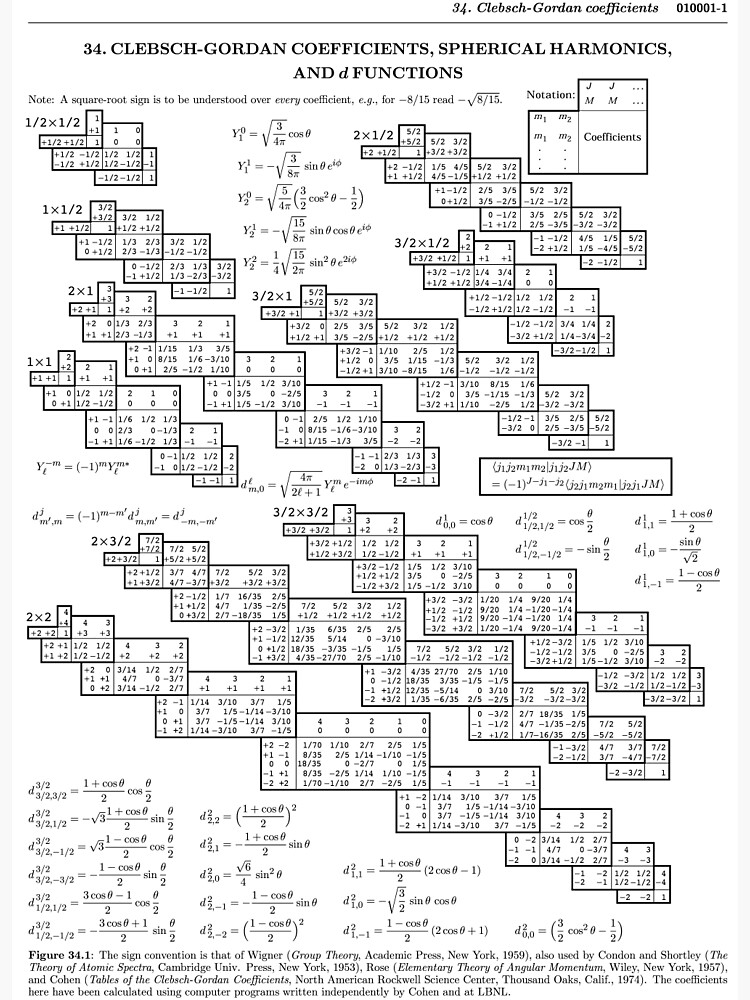
\includegraphics{figs/cl-gord}
	%    \caption{This is a margin figure.}
	\label{fig:cl-gord}
\end{marginfigure}
In figura a lato si può vedere una tabella di coefficienti di
Clebsch-Gordan.

\subsection{Stati quantomeccanici di due particelle identiche}\label{sec:particelle-identiche}

Lo studio dei sistemi quantomeccanici formati da particelle identiche conduce a nuove
sorprendenti proprietà che non trovano alcuna analogia nella fisica
classica.
Vediamo un esempio.

Immaginiamo di essere in ambito macroscopico e quindi soggetti alle
leggi della \emph{fisica classica}.
\begin{marginfigure}
	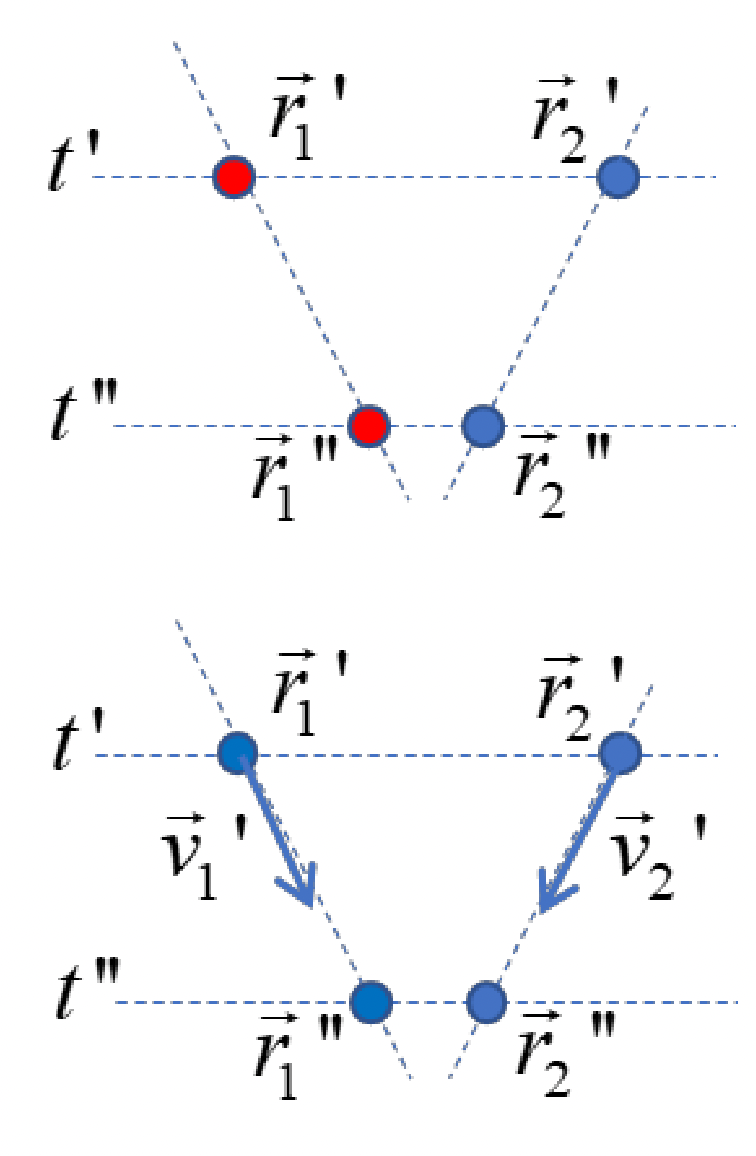
\includegraphics{figs/identical-part1}
	%    \caption{This is a margin figure.}
	\label{fig:identical-part1}
\end{marginfigure}
Immaginiamo poi che, in una certa porzione di spazio, si muovano due
piccole sferette, e che tale spazio sia illuminato ad intervalli di
tempo regolari da una luce stroboscopica.
Il lampo luminoso al tempo
\(t'\) mostrerà le due sferette nelle posizioni \(r_{1}'\) e \(r_{2}'\)
e quello al tempo \(t''\) in \(r_{1}''\) e \(r_{2}''\).
Con tutta
evidenza, se le due sferette sono diverse non esiste alcun problema
nell'associare alle posizioni osservate, in ogni dato istante di tempo,
la specifica sferetta.
Si dice allora che in meccanica classica due
particelle diverse sono sempre distinguibili.

Diverso sembra il caso in cui le due sferette siano identiche.
Infatti,
non sapremmo dire se la sferetta nella posizione \(r_{1}''(r_{2}'')\) al
tempo \(t''\) sia quella che al tempo \(t'\) si trovava in \(r_{1}'\) o
quella che si trovava in \(r_{2}'\).
L'identità delle sferette ci ha
condotti dunque alla impossibilità di associare con certezza le
posizioni alle particelle.
L'ambiguità, però, non è essenziale poichè
può essere superata qualora al tempo t' siano note, non solo le
posizioni delle sferette, ma anche le loro velocità \(v_1'\) e \(v_2'\).
Infatti, al tempo \(t''\) ciascuna sferetta dovrà trovarsi non troppo
lontano dalla direzione della propria velocità al tempo \(t'\) (se
l'istante \(t''\) non è troppo lontano da \(t'\)).
Concludiamo allora
che, se in un istante di tempo le posizioni e le velocità di due
sferette identiche sono note con sufficiente precisione, sarà sempre
possibile determinare la loro posizione in ogni istante di tempo
successivo.

Poiché nella meccanica classica non ci sono limitazioni nel conoscere in
ogni istante di tempo le posizioni e le velocità delle particelle in
gioco, concludiamo che \textbf{nella fisica classica sia le particelle
	diverse che quelle identiche sono sempre distinguibili}.

Cosa accade in meccanica quantistica?
E' semplice rendersi conto che nel
caso di particelle diverse una ipotetica misura di massa, carica o di
una qualunque variabile interna capace di determinarne l'identità sarà
in grado di dirci senza ambiguità quale posizione occupi ciascuna delle
due particelle.
Dunque, analogamente al caso della meccanica classica,
giungiamo quindi ad affermare che nella meccanica quantistica due
particelle diverse sono sempre distinguibili.

Ben diverso è il caso in cui le particelle siano identiche.
Infatti - a
differenza di ciò che accade in meccanica classica -- uno stato
quantomeccanico non può possedere in ogni istate di tempo sia posizioni
definite che velocità definite (principio di indeterminazione).
Se ad
esempio al tempo \(t'\) sono definite le posizioni \(r_{1}'\) e
\(r_{2}'\) delle due particelle identiche, risulteranno allora
indefinite le corrispondenti velocità \(v_{1}'\) e \(v_{2}'\)
pregiudicando dunque la possibilità di attribuire univocamente una
posizione a ciascuna di esse al tempo t'\,. Analogamente, se al tempo
t' sono definite le velocità \(v_{1}'\) e \(v_{2}'\) delle due
particelle identiche (e dunque le quantità di moto), risulteranno allora
indefinite le loro posizioni che non potranno essere univocamente
assegnate alle particelle stesse.

Giungiamo allora a concludere che \textbf{nella meccanica quantistica
	due particelle identiche sono sempre indistinguibili}.
Tale fatto può
essere visto in modo ancor più diretto attraverso il seguente\\
esempio.
Immaginiamo di avere due particelle microscopiche identiche che
si trovino in stati quantomeccanici diversi, ad esempio di quantità di
moto ed energia (\(E_1, p_1\)) ed (\(E_2, p_2\)) descritte da due onde
piane di De Broglie (vedi figura).\\
\begin{marginfigure}
	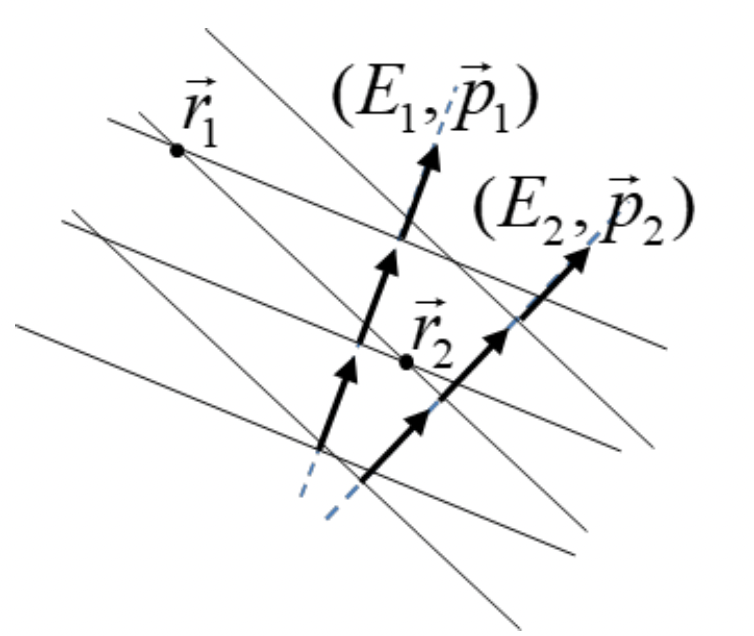
\includegraphics{figs/identical-part2}
	%    \caption{This is a margin figure.}
	\label{fig:identical-part2}
\end{marginfigure}
Con tutta evidenza due misure di posizione potranno trovare la
particella (\(E_{1},p_{1}\)) nella posizione \(r_{1}\) e la particella
(\(E_{2},p_{2}\)) nella posizione \(r_{2}\), oppure la particella
(\(E_{2}, p_{2}\)) nella posizione \(r_{1}\) e la particella
(\(E_{1}, p_{1}\)) nella posizione \(r_{2}\), dando quindi luogo alla
ambiguità discussa.

L'esempio può guidarci anche alla costruzione della funzione d'onda del
sistema quantomeccanico delle due particelle identiche.\\
Per cominciare consideriamo due particelle identiche poste in regioni di
spazio differenti ovvero mutuamente isolate (ad esempio ponendole in
contenitori diversi).
La densità di probabilità di osservare la
particella (\(E_{1},p_{1}\)) nella posizione \(r_{1}\) e la particella
(\(E_{2},p_{2}\)) nella posizione \(r_{2}\) è data allora dal modulo
quadrato della seguente funzione d'onda

\begin{equation}
	\psi_{E_{1},\mathbf{p}_{1}}(\mathbf{r}_{1},t) \psi_{E_{2},\mathbf{p}_{2}}(\mathbf{r}_{2},t)
\end{equation}

dove i termini a prodotto sono le funzioni d'onda delle singole
particelle \begin{gather*}
	\psi_{E_{1},\mathbf{p}_{1}}(\mathbf{r}_{1},t) = A_{E_{1},\mathbf{p}_{1}}e^{ \frac{i}{\hbar} (\mathbf{p}_{1} \cdot \mathbf{r}_{1}-E_{1}t)}\\
	\psi_{E_{2},\mathbf{p}_{2}}(\mathbf{r}_{2},t) = A_{E_{2},\mathbf{p}_{2}}e^{ \frac{i}{\hbar} (\mathbf{p}_{2} \cdot \mathbf{r}_{2}-E_{2}t)}\\
\end{gather*} Se ora rimuoviamo la condizione di isolamento, costruendo un unico
sistema fisico formato da due particelle identiche poste nella stessa
regione di spazio (ad esempio mettendole entrambe nello stesso
contenitore) ci rendiamo subito conto che la funzione d'onda (\(35\))
non descrive lo stato quantomeccanico in modo completo.
Infatti - come
osservato in precedenza -- è anche possibile che una misura di posizione
sul sistema trovi la particella (\(E_{2},p_{2}\)) in \(r_{1}\) e la
particella (\(E_{1},p_{1}\)) in \(r_{2}\), un esito evidentemente non
descritto dalla (\(35\)).
Tale esito è invece descritto dalla seguente
funzione d'onda

\begin{equation}
	\psi_{E_{2},\mathbf{p}_{2}}(\mathbf{r}_{1},t) \psi_{E_{1},\mathbf{p}_{1}}(\mathbf{r}_{2},t)
\end{equation} dove i termini a prodotto sono dati dalle funzioni d'onda
delle singole particelle

\begin{gather*}
	\psi_{E_{1},\mathbf{p}_{1}}(\mathbf{r}_{2},t) = A_{E_{1},\mathbf{p}_{1}}e^{ \frac{i}{\hbar} (\mathbf{p}_{1} \cdot \mathbf{r}_{2}-E_{1}t)}\\
	\psi_{E_{2},\mathbf{p}_{2}}(\mathbf{r}_{1},t) = A_{E_{2},\mathbf{p}_{2}}e^{ \frac{i}{\hbar} (\mathbf{p}_{2} \cdot \mathbf{r}_{1}-E_{2}t)}\\
\end{gather*}
Ora, dato che il sistema di due particelle identiche può dare luogo
ad entrambi gli esiti (\(35\)) e (\(36\)), tali esiti -- in accordo con
i principi generali della meccanica quantistica - dovranno essere
sommati coerentemente.
In assenza di ulteriori prescrizioni, non potremo
che introdurre due generici coefficienti complessi ottenendo uno stato
che - pur soddisfacendo i requisiti richiesti - contiene due
coefficienti arbitrari
\[
	\psi_{sis} = \alpha \, \psi_{E_{1},\mathbf{p}_{1}}(\mathbf{r}_{1},t) \psi_{E_{2},\mathbf{p}_{2}}(\mathbf{r}_{2},t) +
	\beta \, \psi_{E_{2},\mathbf{p}_{2}}(\mathbf{r}_{1},t) \psi_{E_{1},\mathbf{p}_{1}}(\mathbf{r}_{2},t)
\]
una ambiguità nota con il nome di \textbf{degenerazione di scambio}.

%%%%%%%%%%%%%%%%%%%%%%%%%%%%%%%%%%%%%%%%%%%%%%%%%%%%%%%%%%%%%%%%%%%%%%%%%%%%%%%%%%%%%%%%%%%%%%%%%%%%%%%%%%%%%%%%%%%%%%%%
%%%%%%%%%%%%%%%%%%%%%%%%%%%%%%%%%%%%%%%%%%%%%%%%%%%%%%%%%%%%%%%%%%%%%%%%%%%%%%%%%%%%%%%%%%%%%%%%%%%%%%%%%%%%%%%%%%%%%%%%
%%%%%%%%%%%%%%%%%%%%%%%%%%%%%%%%%%%%%%%%%%%%%%%%%%%%%%%%%%%%%%%%%%%%%%%%%%%%%%%%%%%%%%%%%%%%%%%%%%%%%%%%%%%%%%%%%%%%%%%%
\section{Il nucleo come gas di fermioni}\label{sec:il-nucleo-come-gas-di-fermioni}

Il modello a goccia del nucleo - essenzialmente fondato sulla natura a corto raggio delle interazioni forti - riesce a
descrivere alcune proprietà del nucleo tra le quali l’esistenza di una energia di legame con termini di volume, superficie e coulombiano.
Non riesce invece a rendere conto in nessun modo dei termini di asimmetria e accoppiamento, chiaramente richiesti dai
dati sperimentali, ma che devono essere introdotti ‘a mano’ nella formula di Weizsacker.
Tale fatto dimostra che oltre alla natura a corto raggio delle interazioni forti, nel nucleo giocano un ruolo di rilievo
altre proprietà trascurate dal modello a goccia, presumibilmente legate alla natura quantomeccanica dei suoi costituenti.
Il modello nucleare a gas di fermioni introduce nel gioco alcuni essenziali proprietà quantomeccaniche in una forma il
più possibile semplificata.





